\documentclass{article}
\usepackage{ctex}
\usepackage{geometry}
\geometry{top = 2cm, left = 1cm, right = 1cm, bottom = 2cm}
\usepackage{amsmath,amssymb,amsthm,amsfonts}
\usepackage{abstract}
\usepackage{siunitx}
\usepackage{graphicx}
\usepackage{booktabs}
\usepackage{appendix}
\usepackage{hyperref}

\renewcommand{\appendixpagename}{附录}


\title{用正比计数器测量X射线的吸收和特征谱}
\author{钱思天 2001112187}
\begin{document}
    \maketitle
    \begin{abstract}
        本实验利用了正比探测器和多道计数器,对经由$^{238}\text{Pu}$放射源激发的不同样品特征X射线进行了测量。通过对铁、钴、锗、铜、锌等元素的特征X射线测量,
        结合参考$K_\alpha$能谱对多道计数器进行了能量刻度。并利用刻度后的测量系统测量了三个未知样品的特征X射线能量,继而确定了元素种类。而后,通过添加不同厚度的
        铝吸收片的铜特征X射线的测量结果,测得了铝对X射线的线性吸收系数。最后,利用了$^{55}\text{Fe}$的特征X射线的测量结果,评估了正比探测器的分辨本领。
        \newline
        \newline
        {\emph{ 关键词:\ 正比计数器、特征X射线、线性吸收系数 }\rm}

    \end{abstract}

    \section{背景简介}
    \subsection{实验原理}
    \subsubsection{本征$X$射线谱}
    原子核通过核衰变过程(内转换及轨道电子俘获)或由外部射线激发而在其内层产生电子空穴,当外层电子向内层跃迁时发射的射线即为特征$X$射线。玻耳理论指出电子跃迁时放出的光子具有一定的波长$\lambda$,它的能量为:
    \begin{equation}
        h v=Z^{2} \frac{2 \pi^{2} m_{0} e^{4}}{h^{2}}\left(\frac{1}{n_{1}^{2}}-\frac{1}{n_{2}^{2}}\right)
    \end{equation}
其中$n_1$、$n_2$为电子终态、始态所处壳层的主量子数,对$K_\alpha$线系
$n_1=1$,$n_2=2$。根据特征X射线的能量,可以辨认激发原子的原子序数。
    \subsubsection{$X$射线的吸收}
    $X$射线是一种能量较低的电磁波,它的波长在$100\text{\AA}$到$0.01\text{\AA}$之
间。当一束单色$X$射线垂直入射到某种材料上时,通过吸收体后的$X$射线强度将减弱,即$X$射线被物质吸收。它包含吸收和散射两个过程。
吸收过程主要包含光电吸收即光电效应。散射过程包含康普顿散射和汤姆逊散射。

设一厚度及成份均匀的吸收体,其厚度为$t$,每立方厘米有$N$个原子。若能量为$h\nu$的准直光束,单位时间内垂直入射到吸收体单位
面积上的光子数为$I_0$,那么通过厚度为$t$的物质后,透射出去的光子数为$I(t)$,并表示为:
\begin{equation}
    I(t) = I_0\exp(−\mu t) 
\end{equation}

式中$\mu$定义为线性吸收系数,$\mu=N\cdot\sigma$,$\sigma$为截面。

对于铝吸收材料,当$X$射线的能量低于$40\si{KeV}$时,光电效应占优势,康普顿散射可以忽略。光电效应的线性吸收系数为
\begin{equation}
    \mu_m = \frac{\mu}{\rho}(\si{cm^2\per g})=\phi_0 Z^5 \alpha^42^{5/2}(m_0c^2/h\nu)^{7/2}\frac{N_A}{A}
\end{equation}
式中,$\phi_0 = \frac{8}{3}\pi r_0^2, r_0 = \frac{e^2}{m_0c^2},\alpha\sim\frac{1}{137}$,而$N_A$是阿伏伽德罗常数,$A$是原子量。将铝元素代入,得
\begin{equation}
    \mu_m^{\text{Al}} = 52.694\si{cm^2\per g}
\end{equation}
\subsubsection{正比计数器}
正比计数器可将入射粒子(低能$\gamma$或$X$射线)产生的初电离效应
放大很多倍之后输出,并且输出信号的幅度仍然保持与初电离事件数目成正比,所以正比计数器不仅可以测量计数,还可以用来测量射线能量。由于正比计数管输出脉冲信号幅度比较大,而其本身噪声较小,
因此正比计数管可看成是一个没有噪声的理想放大器。这个特点决定了正比计数器在测量低能粒子方面有其独特的优势,广泛用于测量低
能$\gamma$射线和$X$射线的强度和能量。

正比计数器的能量分辨不仅受到由于原初电离的正负电荷对数
涨落的影响,还受气体放大倍数的影响,所以同样条件下,能量分辨要比$\text{Si}$($\text{Li}$)$X$射线谱仪差。
    \subsection{实验目的}
    \begin{enumerate}
        \item 学习使用正比计数器并熟悉其工作原理;
        \item 了解$X$射线与物质的相互作用原理、掌握其吸收规律;
        \item 利用元素特征$X$射线能量做探测器系统的刻度,并推断未知样品元素种类;
        \item 探测已知种类样品的特征$X$射线谱,评价实验探测系统的分辨率。
    \end{enumerate}
    \section{实验操作}
    \subsection{实验装置}
    实验装置示意图如图\ref{fig:ExpIns}。涉及的实验装置如下:
    \begin{figure}[htbp]
        \centering
        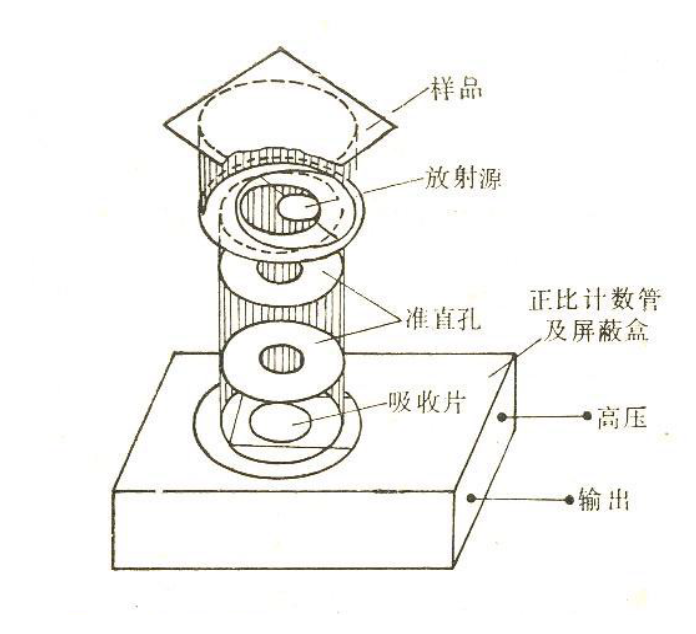
\includegraphics[width=0.7\textwidth]{../plot/ExpIns.png}
        \caption{实验装置示意图\label{fig:ExpIns}}
    \end{figure}
    \begin{enumerate}
        \item 正比计数器:一套;
        \item 电荷灵敏前置放大器(放大倍率:$\times 5$):一个;
        \item 插件式高压电源、低压电源、主放大器:各一个;
        \item NIM机箱:一个;
        \item 多道数据采集及微机系统:一套;
        \item 样品(铜等):若干;
        \item 铝吸收片:若干;
        \item $^{238}\text{Pu}$放射源:一枚;
        \item $^{55}\text{Fe}$放射源:一枚。
    \end{enumerate}
    \subsection{实验操作}
    \begin{enumerate}
        \item 观察已安装好的测量$X$射线的探头结构,连接仪器并预热(注
        意先开偏压,后加高压)。打开微机,进入微机多道数据采集系统。
        \item 逐渐升高正比计数器的高压至额定值约2000V,放大倍率设置为$0.9 \times 200 $倍。
        \item 用微机多道测量$^{238}\text{Pu}$源激发的五种已知样品的特征$X$射线谱(探测时间为$600\si{s}$)并
        确定其峰位。从附录特征$X$射线及吸收限表中查出各样品对应
        的$X$射线能量,作峰位道数-能量关系曲线。 
        \item 测量三个未知样品的特征$X$射线谱(探测时间为$600\si{s}$),根据能量刻度结果确定样
        品元素种类。
        \item 测量铜样品的特征$X$射线谱,并选定适当的阈值和道宽来确定
        峰面积计算范围。选择5个不同层数的铝吸收片(每片铝箔厚$2.15\si{mg\per cm^2}$),插在射线和探测器之间的插槽里,测量对应的铜样品的特征$X$射线强度(探测时间为$1200\si{s}$)。
        \item 对所测得的一组数据结果进行最小二乘法拟合,求出吸收系数$\mu_m$。
        \item 用微机多道对$^{55}\text{Fe}$源进行能谱测量,评价能量分辨率。
    \end{enumerate}
    \section{数据处理}
    \subsection{利用已知样品标定探测器,并确定未知样品的元素}
    对于铁、铬、铜、锌、锗五种样品的测量结果(如图\ref{fig:Calibration})
    \begin{figure}
        \centering
        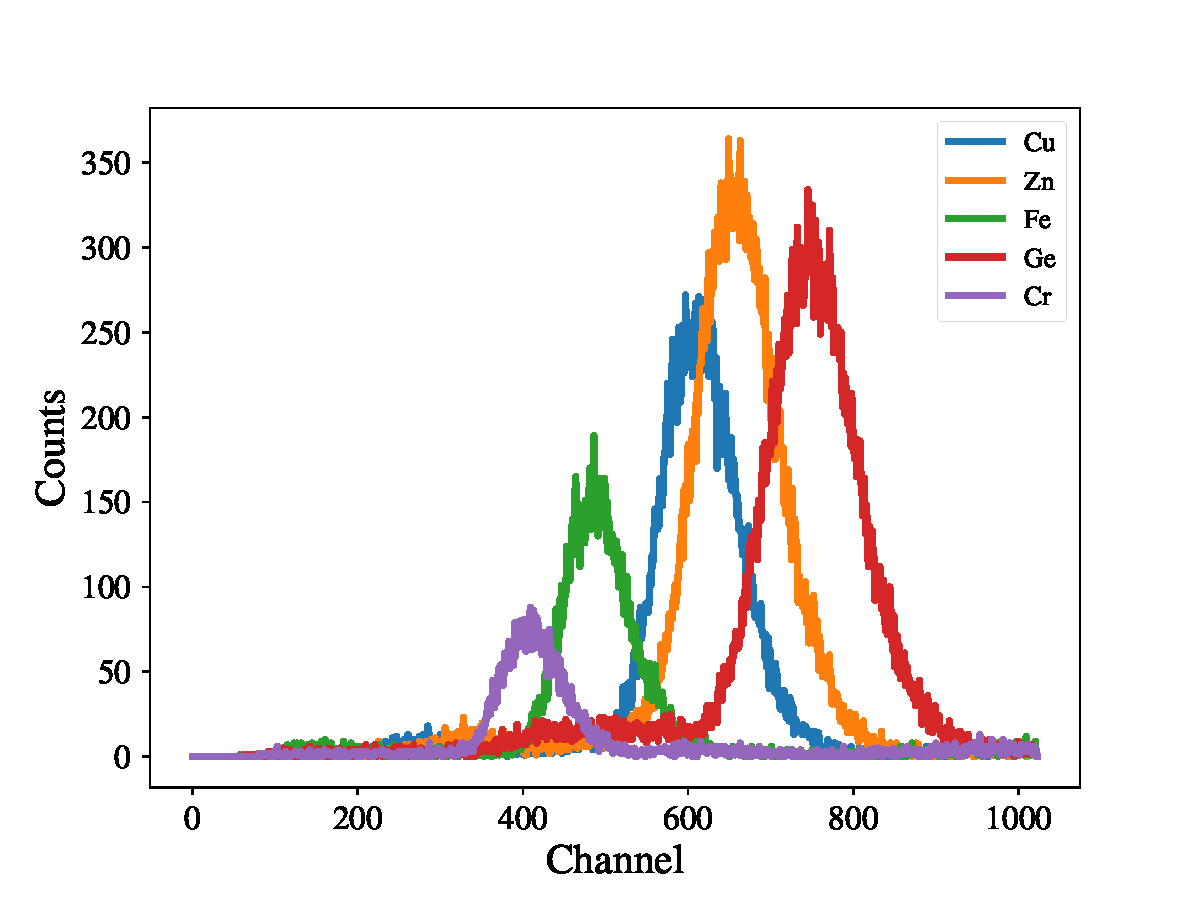
\includegraphics[width=0.7\textwidth]{../plot/Calibration.pdf}
        \caption{五种样品的特征$X$射线谱测量结果\label{fig:Calibration}}
    \end{figure}
    进行高斯拟合(拟合图见附录),得到的峰位如下表\ref{tab:Calibration}
    \begin{table}[htbp]
        \centering
        \caption{五种样品的特征$X$射线谱拟合峰位及参考$K_\alpha$系能量\label{tab:Calibration}}
        \begin{tabular}{lrrrrr}
            \toprule
            {} &          Cu &          Zn &          Fe &          Ge &          Cr \\
            \midrule
            Fitted Peak Pos. &  613.17 &  658.92 &  488.21 &  750.43 &  410.70 \\
            $K_\alpha[\si{KeV}]$ &    8.047 &    8.638 &    6.403 &    9.885 &    5.414 \\
            \bottomrule
            \end{tabular}
    \end{table}
    根据多道探测器的道址与能量的线性关系,利用最小二乘法进行线性回归做刻度,得到刻度关系为:
    \begin{equation}
        E = 0.0131*\text{Ch} - 0.0030
    \end{equation}
    回归表现极佳,$R^2=0.9999$。结合对未知实验的测量结果(见图\ref{fig:Prediction},拟合图见附录),可得表\ref{tab:Prediction}。
    \begin{figure}[htbp]
        \centering
        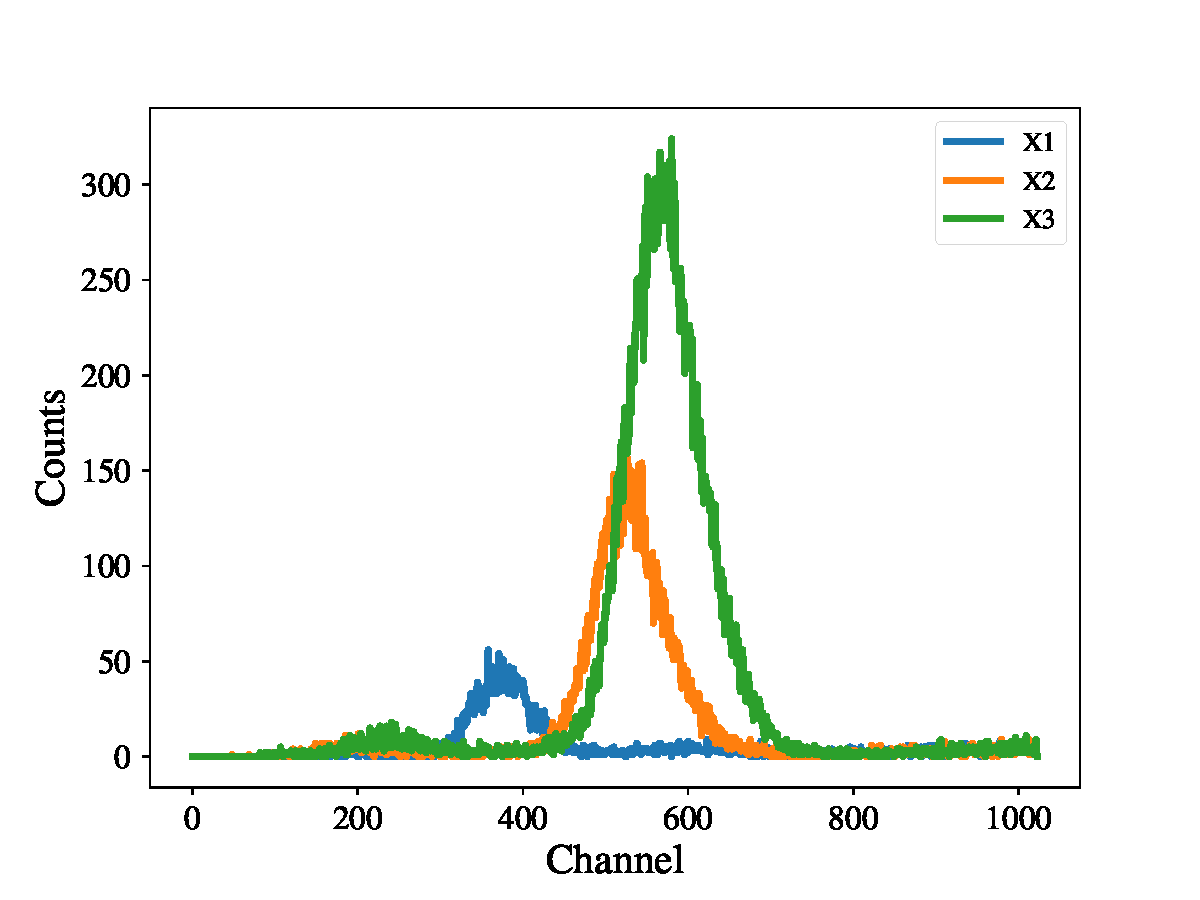
\includegraphics[width=0.7\textwidth]{../plot/Prediction.pdf}
        \caption{三种未知样品的特征$X$射线谱\label{fig:Prediction}}
    \end{figure}
    \begin{table}[htbp]
        \centering
        \caption{三种未知样品的特征$X$射线谱高斯峰拟合峰位和$K_\alpha$线系能量预测值\label{tab:Prediction}}
        \begin{tabular}{lrrr}
            \toprule
            {} &          X1 &          X2 &          X3 \\
            \midrule
            Fitted Peak Pos. &  375.41 &  527.96 &  569.94 \\
            $K_\alpha[\si{KeV}]$ &    4.93 &    6.94 &    7.49 \\
            \bottomrule
            \end{tabular}
            
    \end{table}
    和元素$K_\alpha$线系的参考能量对照,确认各未知样品的元素种类如下:
    \begin{enumerate}
        \item X1:V,钒元素;
        \item X2:Co,钴元素;
        \item X3:Ni,镍元素。
    \end{enumerate} 
    本部分的拟合峰位线性回归图及预测$K_\alpha$值如图\ref{fig:LinearReg1}。
    \begin{figure}[htbp]
        \centering
        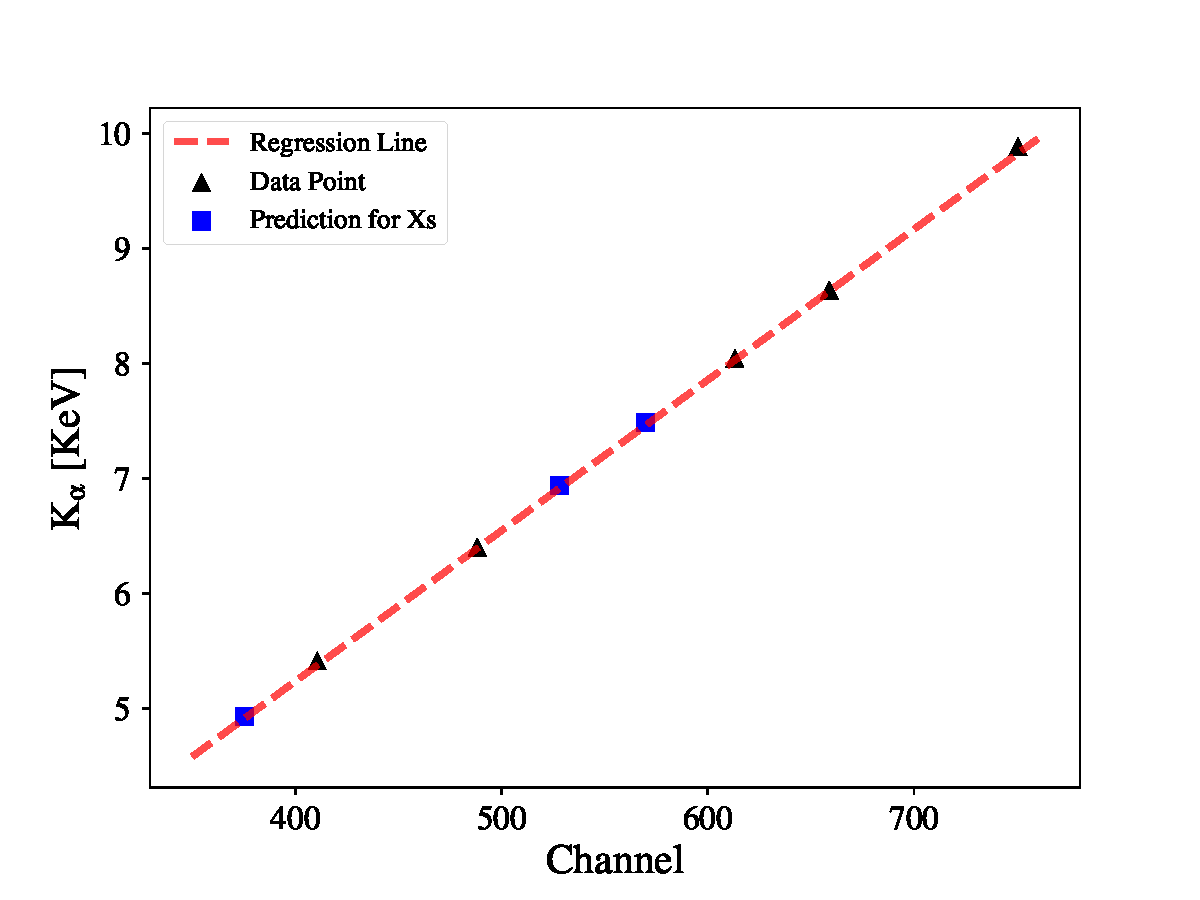
\includegraphics[width=0.7\textwidth]{../plot/LinearReg1.pdf}
        \caption{峰位-$K_\alpha$能级拟合图\label{fig:LinearReg1}}
    \end{figure}
    \subsection{铝片对铜的特征$X$射线线性吸收系数}
    对于不同厚度的铝片,测量结果如图\ref{fig:Absorption}所示(高斯峰拟合结果见附录)。峰拟合结果总结如表\ref{tab:Absorption}。
    \begin{figure}[htbp]
        \centering
        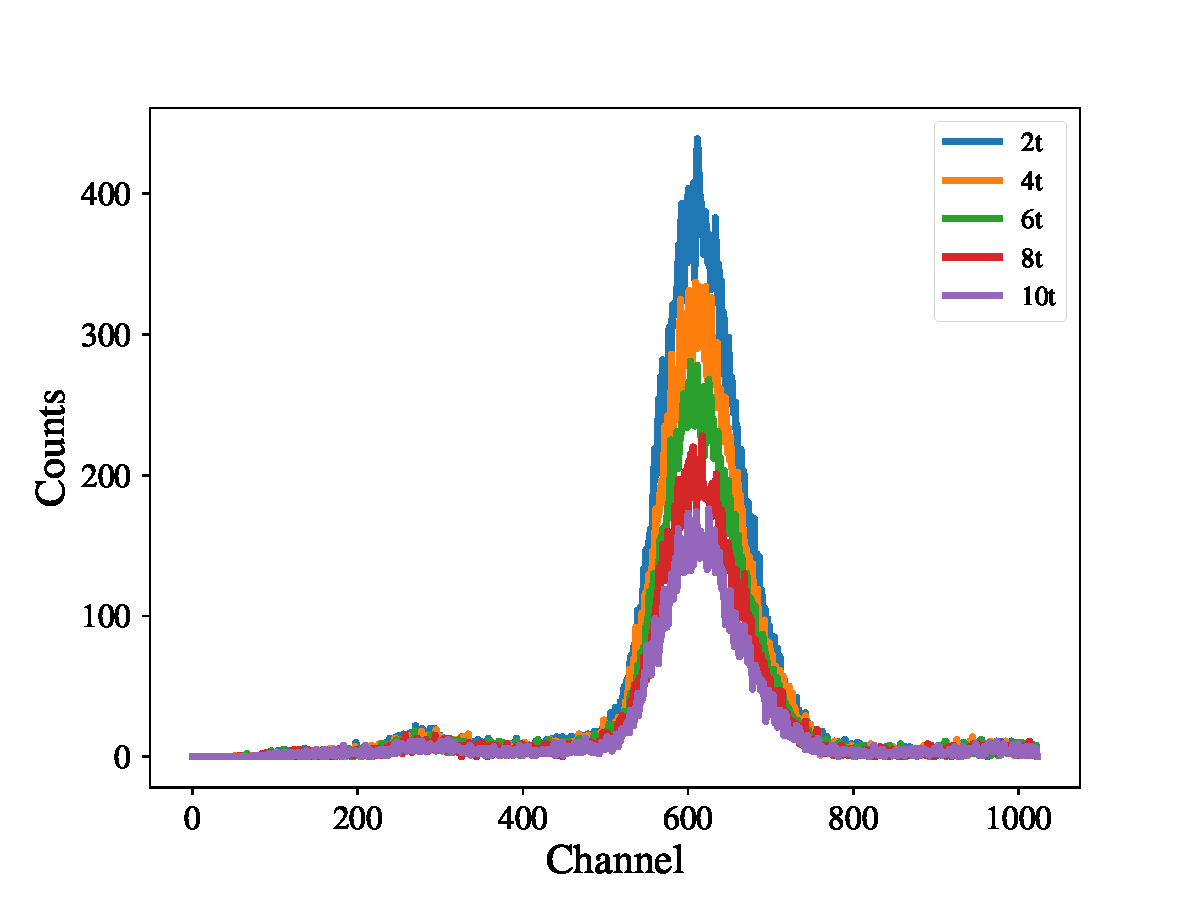
\includegraphics[width=0.7\textwidth]{../plot/Absorption.pdf}  
        \caption{使用不同厚度的铝吸收片后的铜特征$X$射线谱测量结果\label{fig:Absorption}}
    \end{figure}
    \begin{table}[htbp]
        \centering
        \caption{不同厚度的铝吸收片后拟合结果\label{tab:Absorption}}
        \begin{tabular}{lrrrrr}
            \toprule
            Num. of Slices &            2 &            4 &            6 &            8 &           10 \\
            \midrule
            Fitted Peak Pos. &    613.56 &    613.83 &    614.25 &    615.01 &    614.50 \\
            Fitted Stderr.   &     46.47 &     46.53 &     45.90 &     47.39 &     47.63 \\
            Fitted Norm.    &  44897.09 &  35904.35 &  28660.19 &  23116.89 &  18097.90 \\
            Deepth $d_m[\si{mg\per cm^2}]$  &      4.30 &      8.60 &     12.90 &     17.20 &     21.50 \\
            \bottomrule
            \end{tabular}
    \end{table} 
    选取半高峰位(FWHM)下的面积为计数,则有
    \begin{equation}
        S_{\pm \text{FWHM}} = \text{Norm.}*\text{erf}{(\sqrt{2}\ln{2})} \propto \text{Norm.} 
    \end{equation}
    考虑线性吸收下$S\propto S_0*\exp(-\mu_m*d_m)$,则有:
    \begin{equation}
        \ln{(\text{Norm.})} = -\mu_m*d_m+C
    \end{equation}
    进行线性回归(见图\ref{fig:LinearReg2},
    \begin{figure}[htbp]
        \centering
        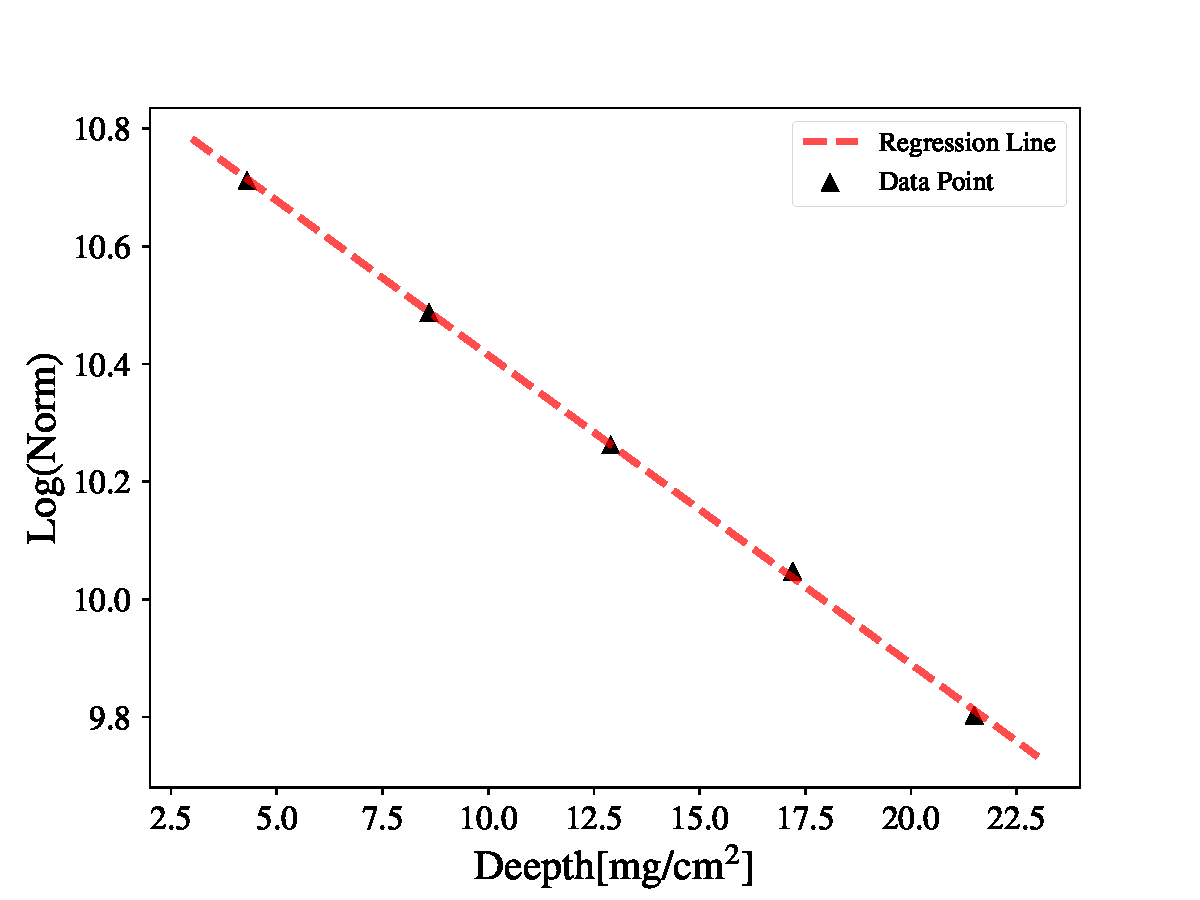
\includegraphics[width=0.7\textwidth]{../plot/LinearReg2.pdf}
        \caption{厚度与拟合归一化系数对数的线性拟合\label{fig:LinearReg2}}
    \end{figure}
    可以得到
    \begin{equation}
        \ln{(\text{Norm.})} = -0.0525*d_m+10.9404 
    \end{equation}
    回归$R^2 = 0.9996$,得到
    \begin{equation}
        \mu_m = -0.0525\si{cm^2\per mg} = -52.5\si{cm^2\per g}
    \end{equation}
    与理论结果符合较好。
    \subsection{利用$^{55}\text{Fe}$对探测器分辨率进行评估}
    对$^{55}\text{Fe}$的测量结果如图\ref{fig:55Fe}。
    \begin{figure}
        \centering
        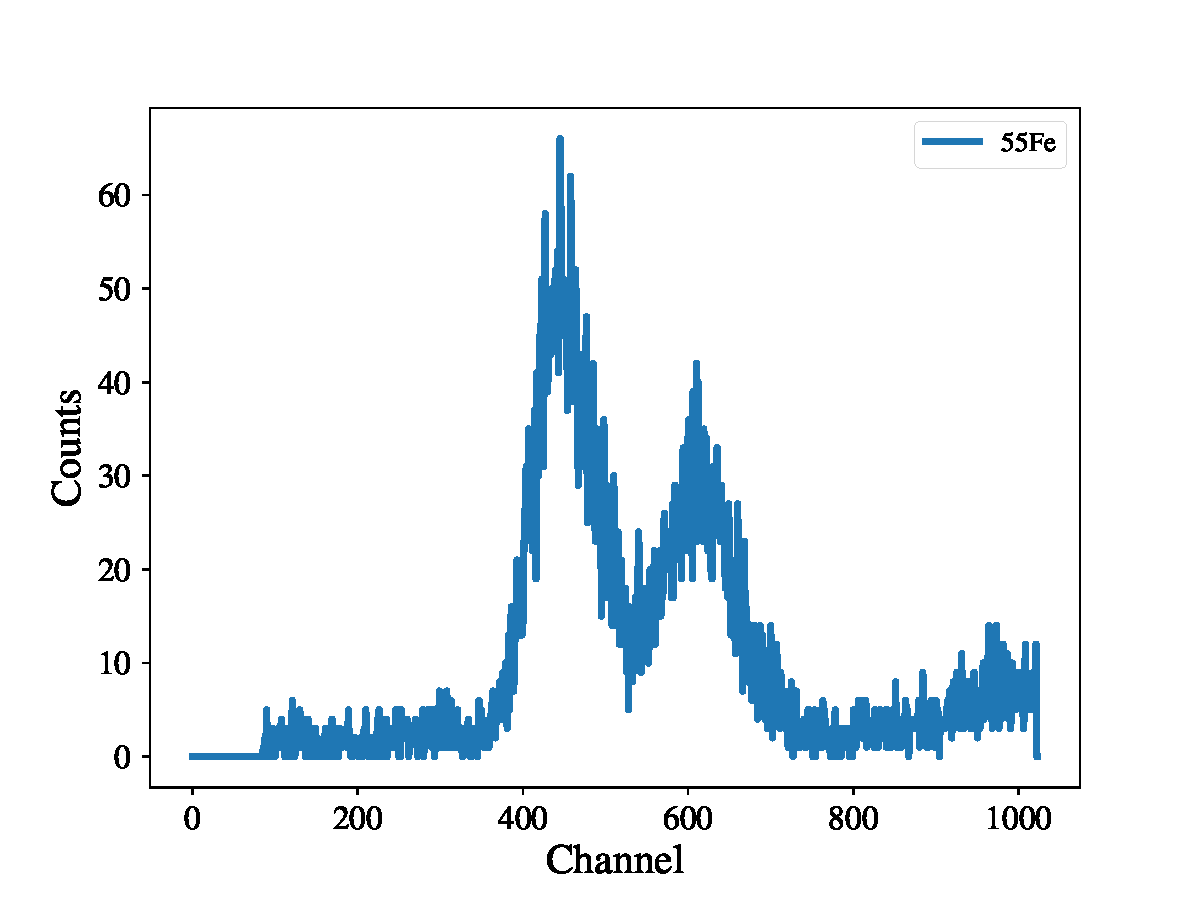
\includegraphics[width=0.7\textwidth]{../plot/55Fe.pdf}
        \caption{对$^{55}\text{Fe}$放射源的测量结果\label{fig:55Fe}}
    \end{figure}
    根据$^{55}\text{Fe}$的原子序数,可以确定其特征$X$射线峰应该是靠左的较高峰。但是,测量结果中存在两个靠的很近的峰,仅仅采用单高斯峰拟合无法解决问题。因此这里采用直接读数的方式进行分辨率评估。
    \begin{table}[htbp]
        \centering
        \caption{$^{55}\text{Fe}$特征$X$射线峰读数结果\label{tab:55Fe}}
        \begin{tabular}{ccccc}
            \toprule
            Peak Pos. &  Left Half Max. & Right Half Max.   &     FWHM        &       Resolution  \\
            \midrule
            444  &      407 &     489 &     82 &    18.4\% \\
            \bottomrule
            \end{tabular}
    \end{table} 
    直接读数的结果给出的分辨率大约在$\mathcal{O}(10\%)$。可见,本实验装置至少在对于$^{55}\text{Fe}$的特征谱测量上,分辨能力较差。当然,从计数来看,可能是因为对于活性较差的$^{55}\text{Fe}$采集时间较短($800\si{s}$)的缘故。这一点也可以从铝吸收系数测量实验中得到印证(见图\ref{fig:Absorption}与图\ref{fig:fitted_sigma}):对于不同厚度的吸收片,FWHM变化不大,但是计数却差异很大。
    \begin{figure}[htbp]
        \centering
        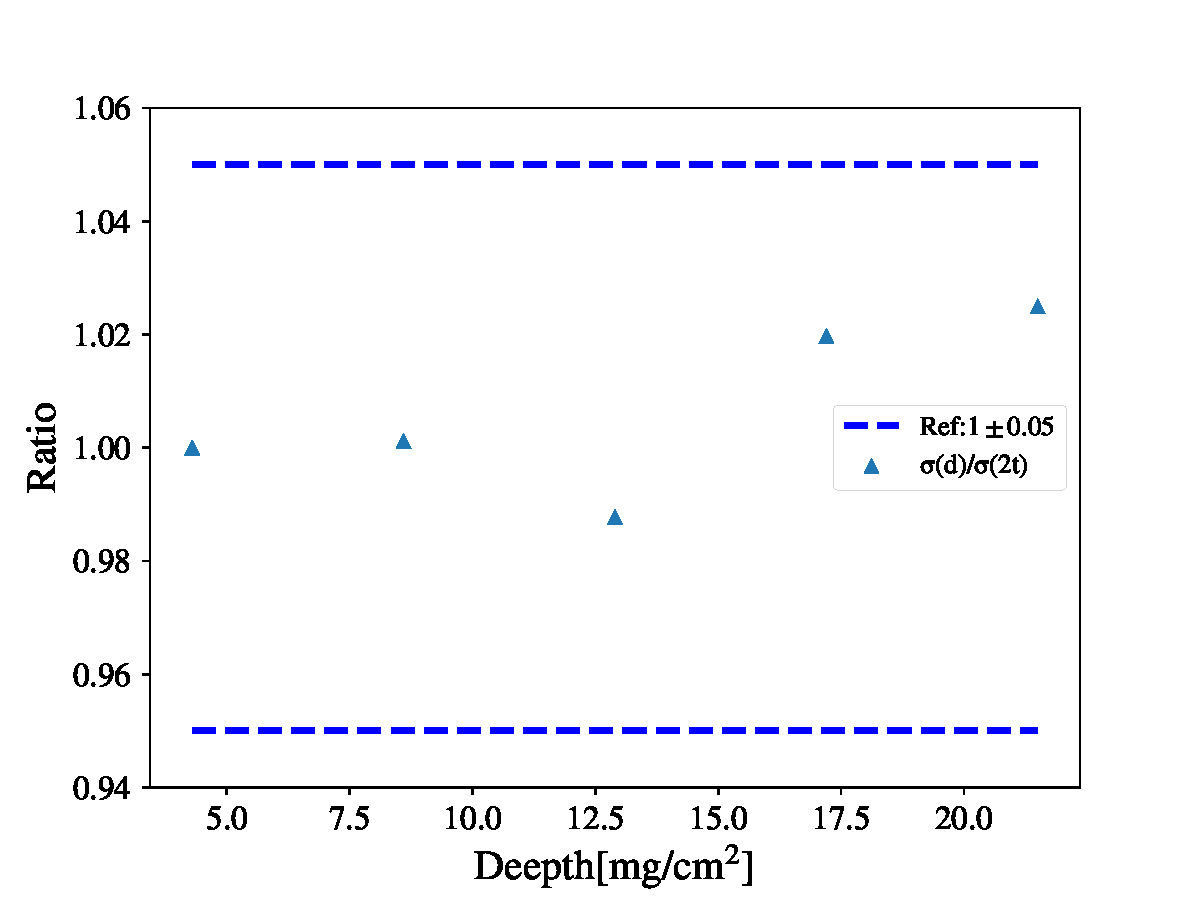
\includegraphics[width=0.7\textwidth]{../plot/fitted_sigma.pdf}
        \caption{不同吸收片厚度的拟合峰宽度比较(以厚度为两片为基准)\label{fig:fitted_sigma}}
    \end{figure}
    \section{结论}
    本实验通过利用五种已知元素样品,对探测器进行了刻度,利用刻度后的探测器探测了三种未知样品的特征$X$射线能量,并鉴别出三种未知样品分别为钒、钴和镍元素。而后,利用实验装置测量了通过不同厚度的铝吸收片的铜特征$X$射线谱,并计算峰面积,得到铝对铜的特征$X$射线线性吸收系数约为$52.5\si{cm^2\per g}$。最后,利用$^{55}\text{Fe}$测量,得到针对其的分辨率约为$19.4\%$。
    \section{致谢}
    感谢许金艳老师的实验指导,感谢刘寅绅同学的讨论。也感谢张轩豪和童星昱同学一起进行实验和借我U盘。
    \clearpage
    \appendix
    \appendixpage
    \section{思考题}
    \begin{enumerate}
        \item 查阅资料得知,$\text{Ag}$的$K_\alpha$能级在$22.162\si{KeV}$,刚好超过了$^{238}\text{Pu}$的激发能力。
        \item 约化后,得到$\sigma_{ph} \propto Z^5(m_0)^{3/2}$,为让吸收系数尽量小,探测器入射窗需要采用较轻的元素。
        \item 考虑角度发散($\theta$),则在材料中的路径会延长为$(d/\cos\theta)$,因此相应的,测得的$\hat{\mu}_m$与实际值$\mu_m$为 $\hat{\mu}_m= \mu_m/\cos\theta$。假设发散角为$10^\circ,25^\circ$,得到修正因子不会超过$1/0.98,1/0.90$,即影响$\sim 2\%,10\%$。
        \item 观察波形,我认为最主要的误差来源还是在信号的强度。波形的展宽比较稳定,提高分辨率的话需要提高峰值。
    \end{enumerate}
    \section{谱线高斯峰拟合结果图}
    \begin{figure}[htbp]
        \centering
        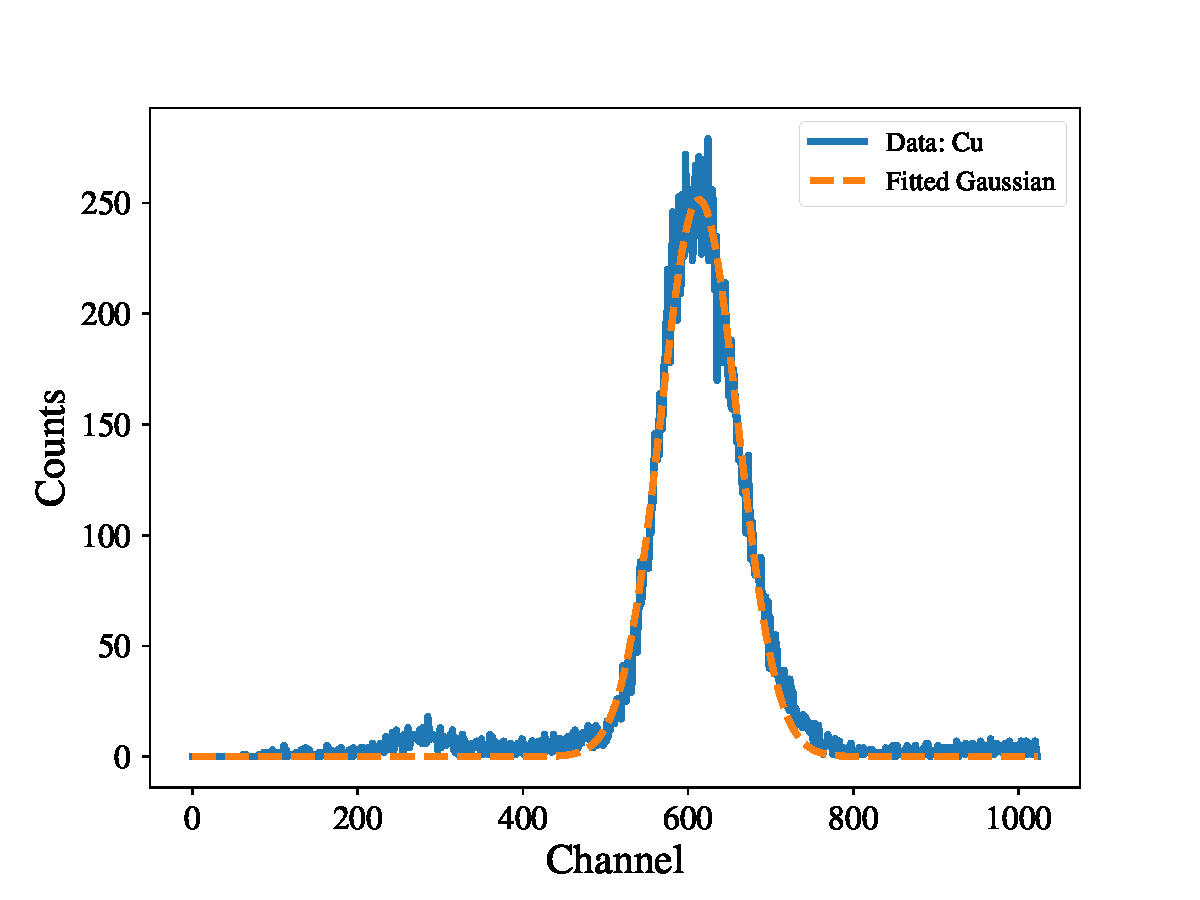
\includegraphics[width=0.7\textwidth]{../plot/Fitted_Cu.pdf}
        \caption{铜样品拟合图\label{fig:Fitted_Cu}}
    \end{figure}
    \begin{figure}[htbp]
        \centering
        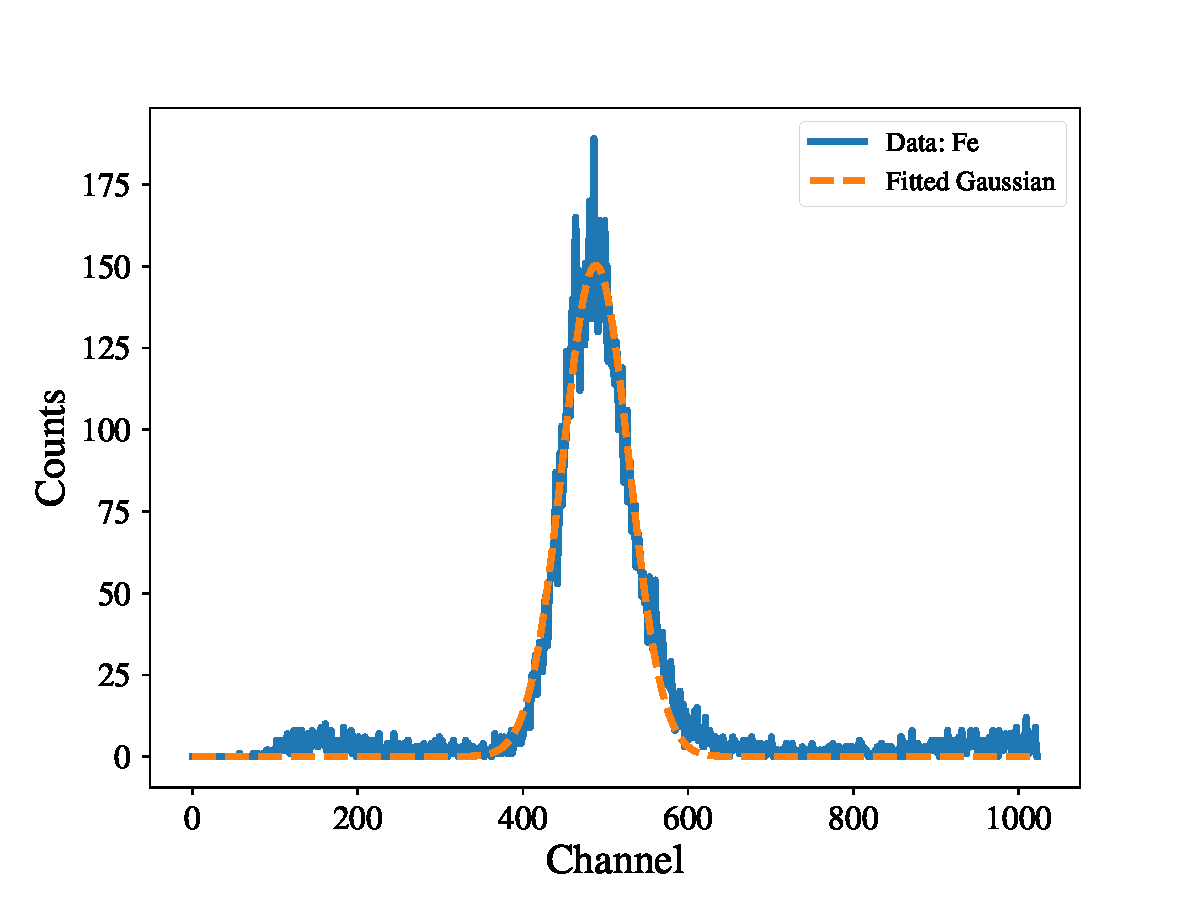
\includegraphics[width=0.7\textwidth]{../plot/Fitted_Fe.pdf}
        \caption{铁样品拟合图\label{fig:Fitted_Fe}}
    \end{figure}
    \begin{figure}[htbp]
        \centering
        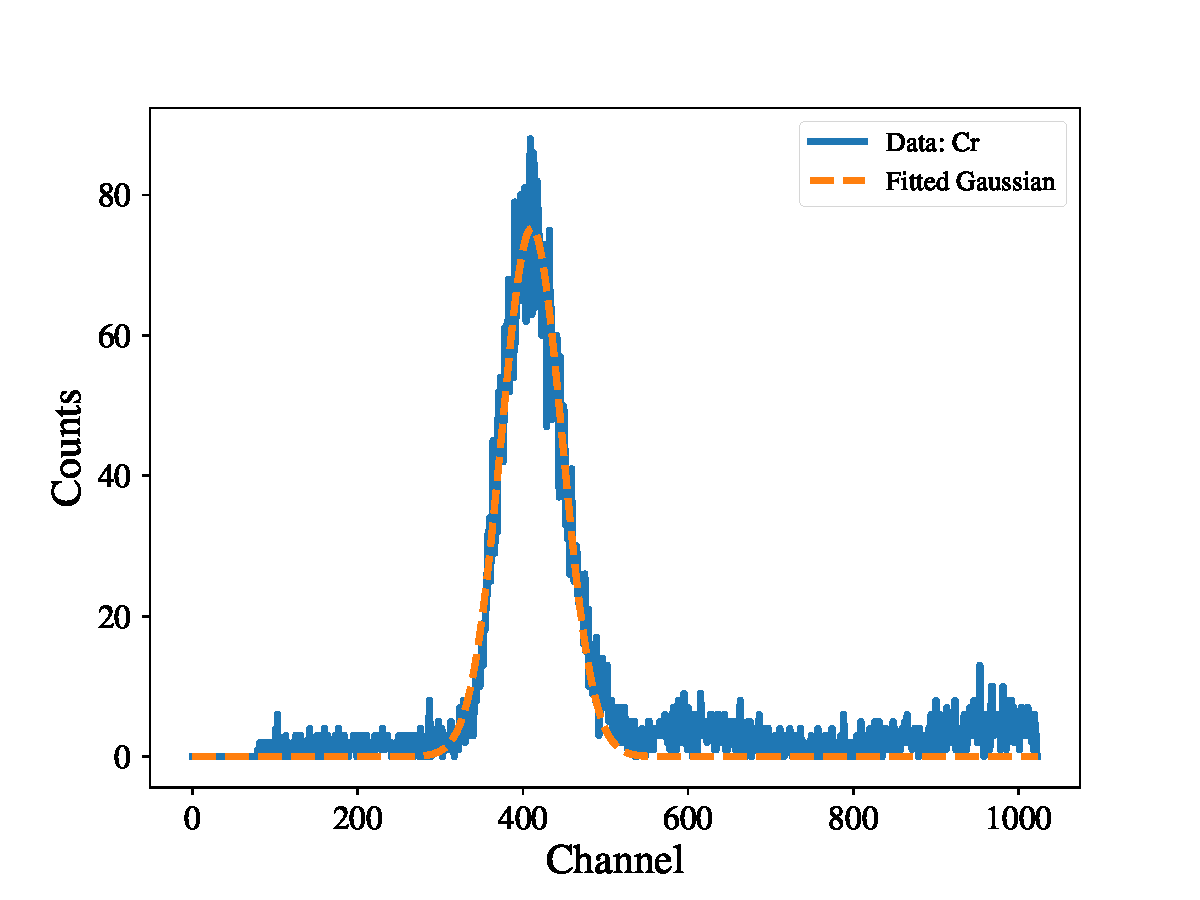
\includegraphics[width=0.7\textwidth]{../plot/Fitted_Cr.pdf}
        \caption{铬样品拟合图\label{fig:Fitted_Cr}}
    \end{figure}
    \begin{figure}[htbp]
        \centering
        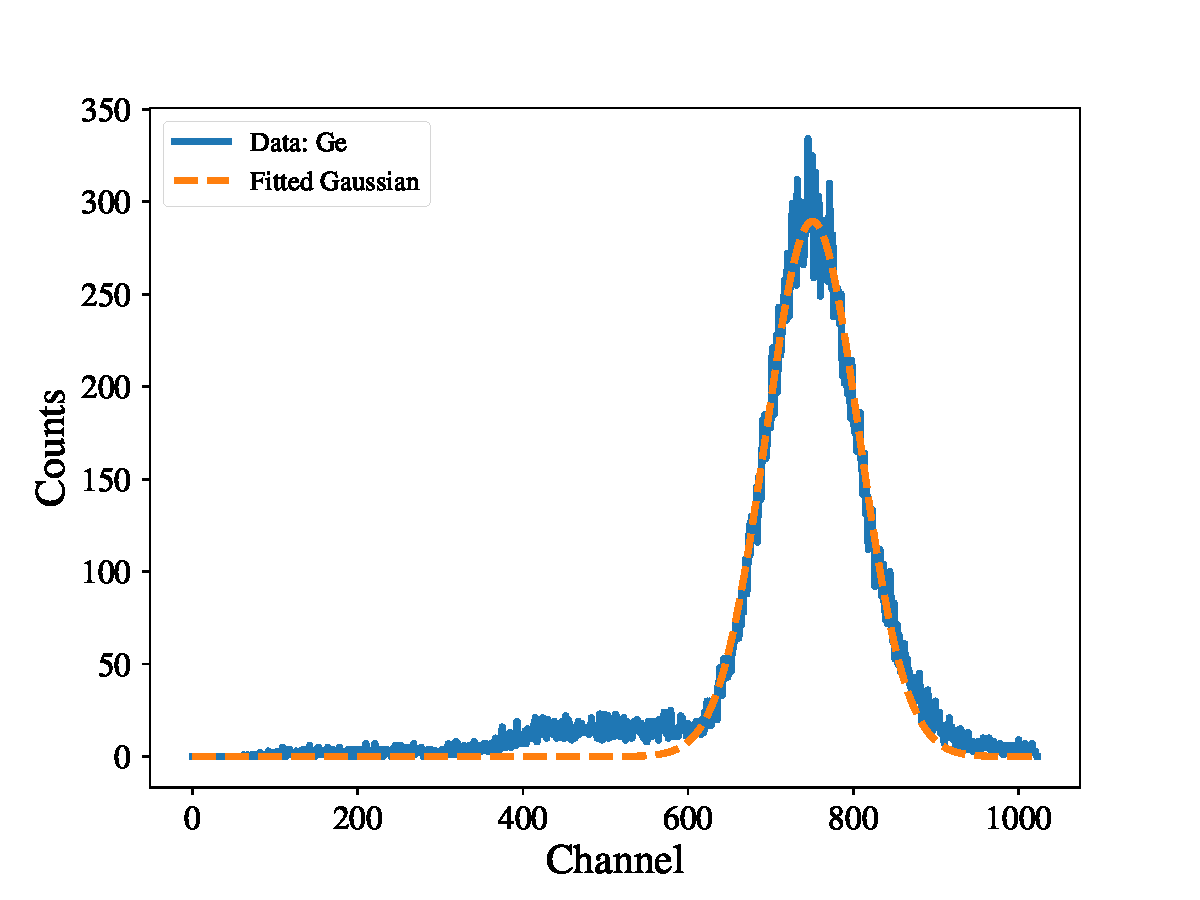
\includegraphics[width=0.7\textwidth]{../plot/Fitted_Ge.pdf}
        \caption{锗样品拟合图\label{fig:Fitted_Ge}}
    \end{figure}
    \begin{figure}[htbp]
        \centering
        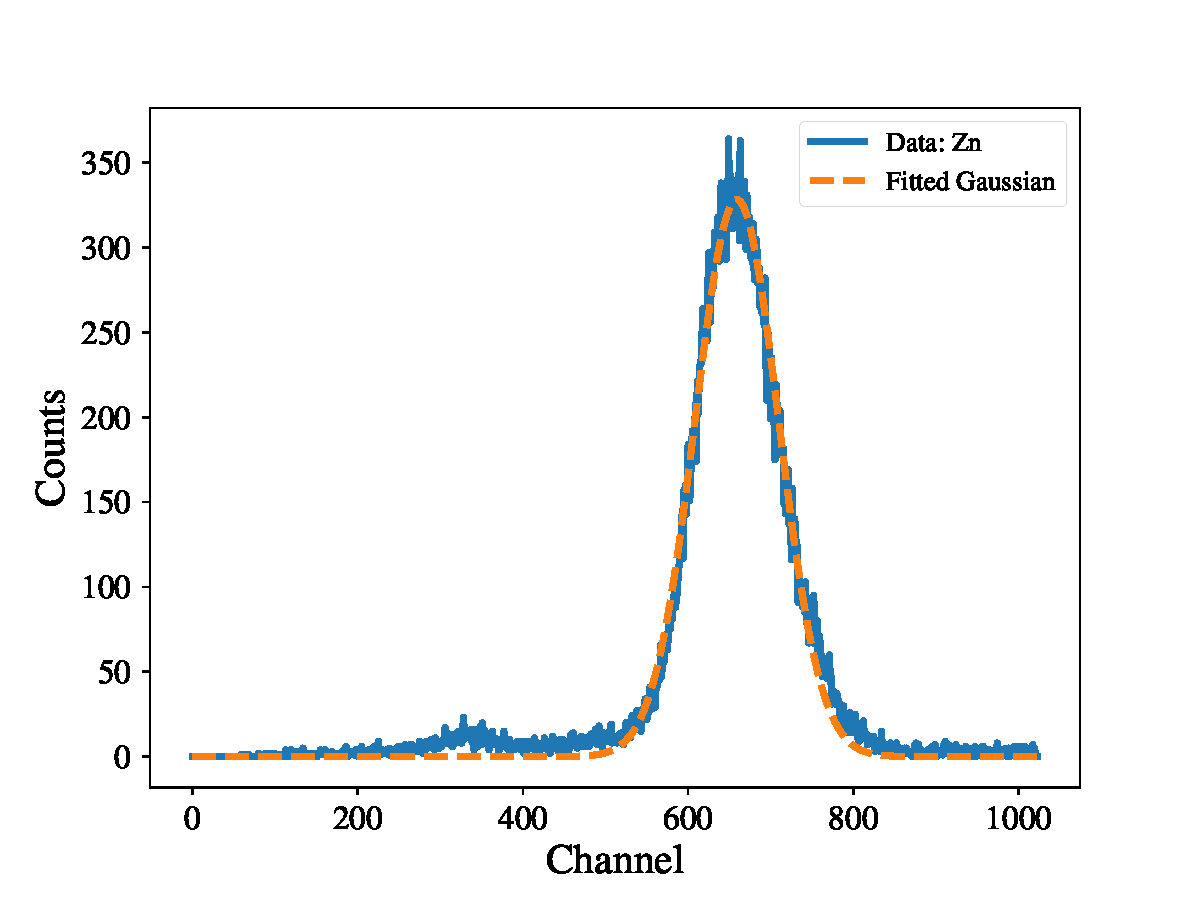
\includegraphics[width=0.7\textwidth]{../plot/Fitted_Zn.pdf}
        \caption{锌样品拟合图\label{fig:Fitted_Zn}}
    \end{figure}
    \begin{figure}[htbp]
        \centering
        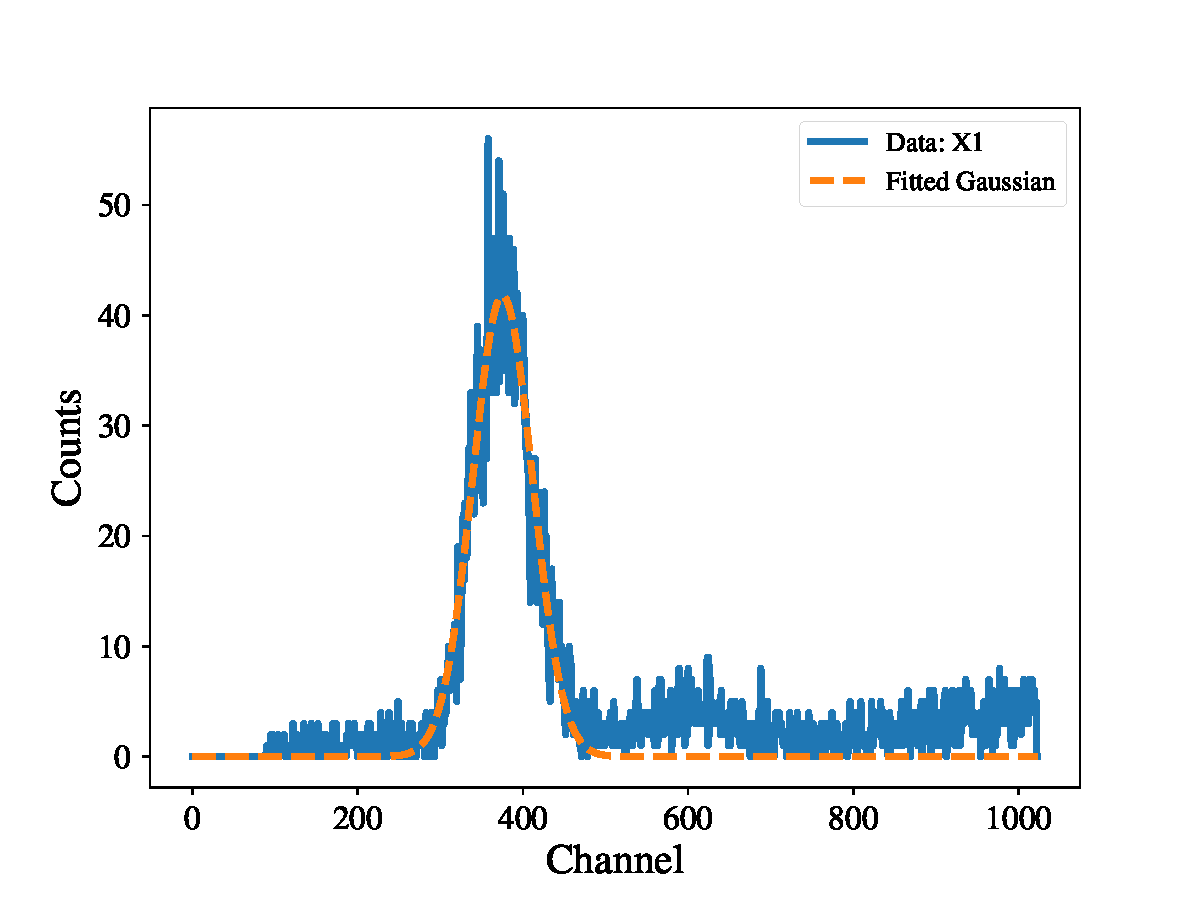
\includegraphics[width=0.7\textwidth]{../plot/Fitted_X1.pdf}
        \caption{未知样品1拟合图\label{fig:Fitted_X1}}
    \end{figure}
    \begin{figure}[htbp]
        \centering
        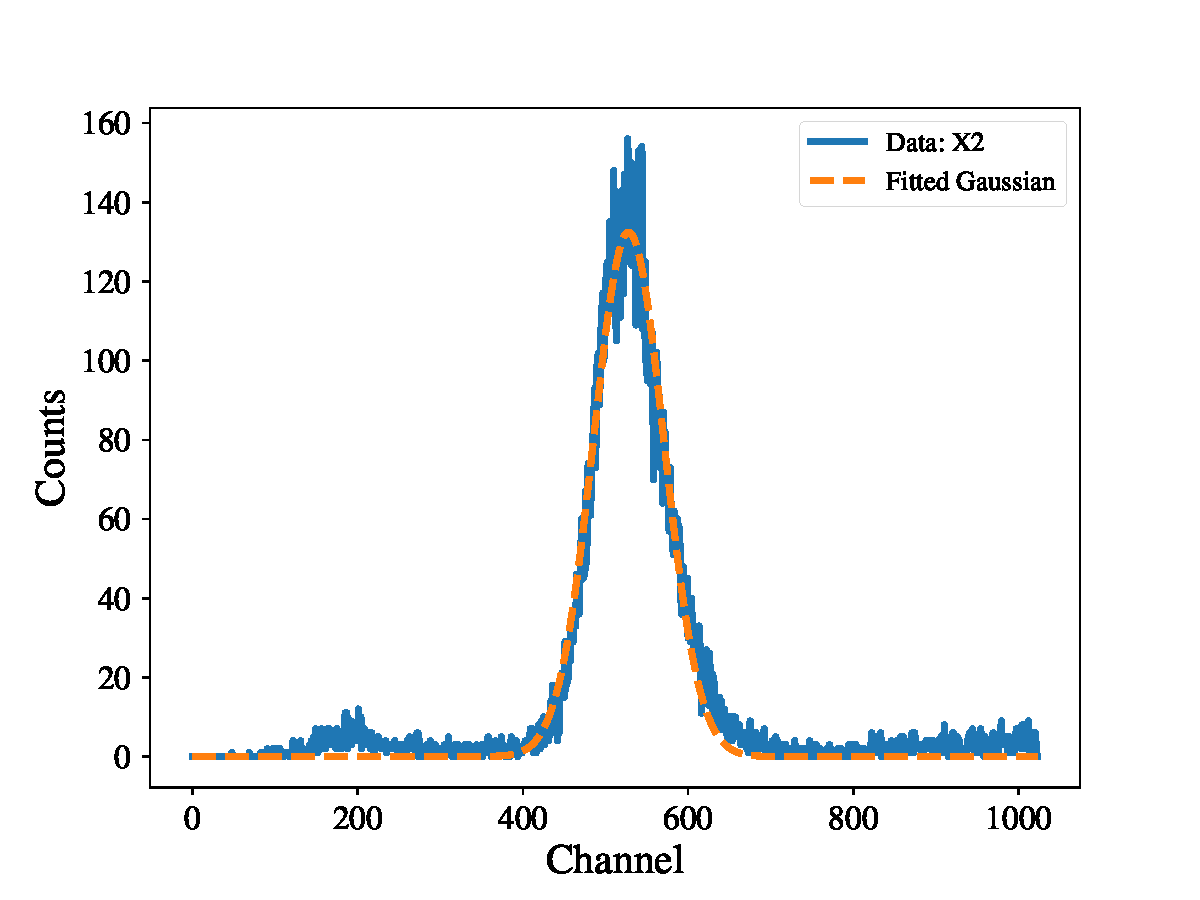
\includegraphics[width=0.7\textwidth]{../plot/Fitted_X2.pdf}
        \caption{未知样品2拟合图\label{fig:Fitted_X2}}
    \end{figure}
    \begin{figure}[htbp]
        \centering
        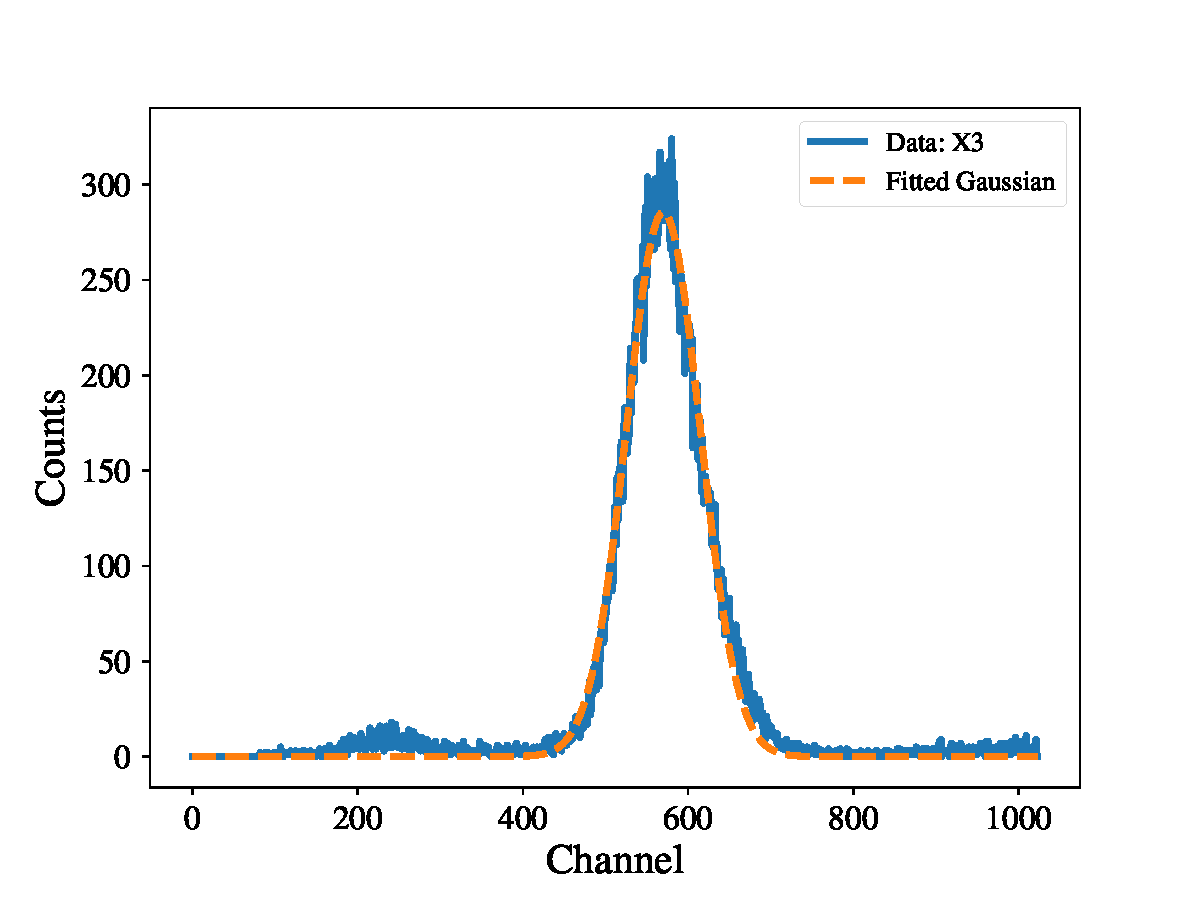
\includegraphics[width=0.7\textwidth]{../plot/Fitted_X3.pdf}
        \caption{未知样品3拟合图\label{fig:Fitted_X3}}
    \end{figure}
    \begin{figure}[htbp]
        \centering
        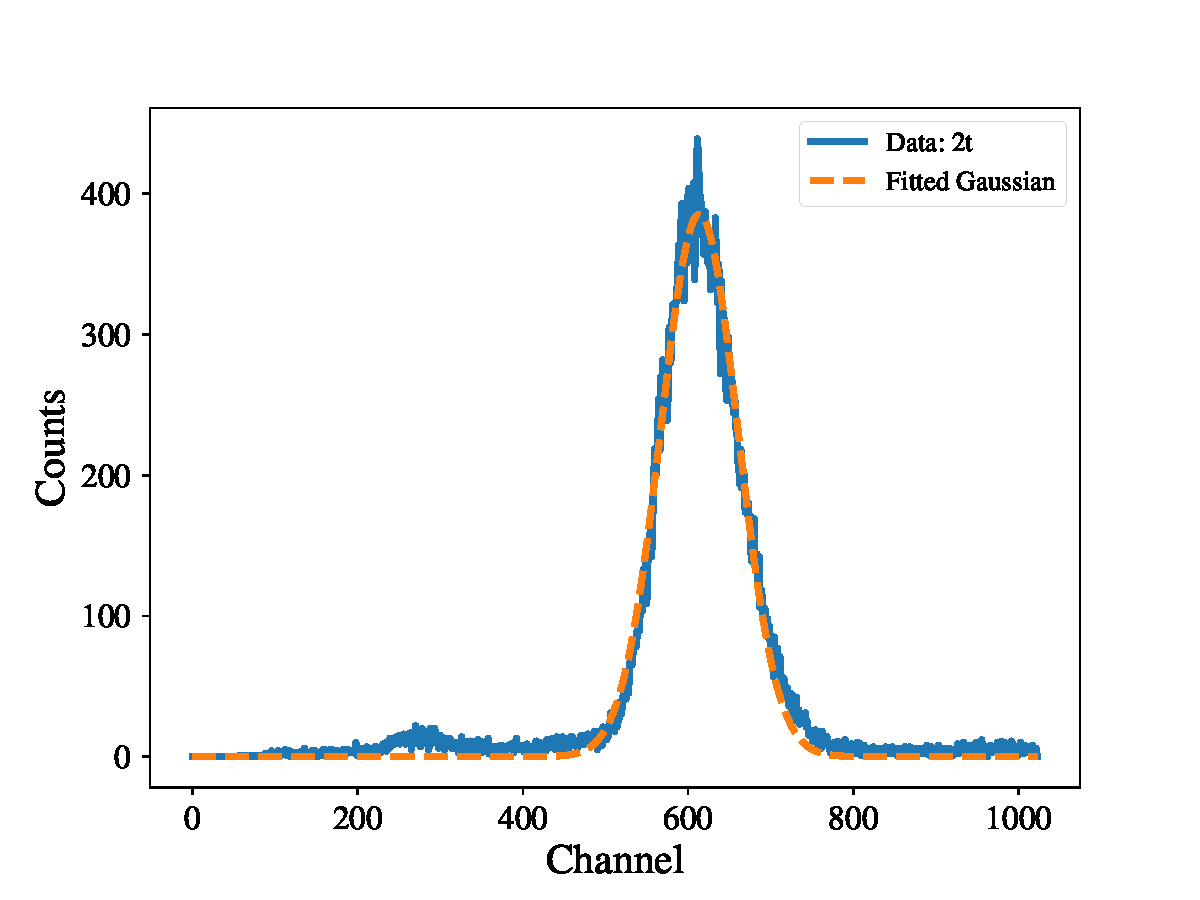
\includegraphics[width=0.7\textwidth]{../plot/Fitted_2t.pdf}
        \caption{2片铝吸收片测量结果拟合图\label{fig:Fitted_2t}}
    \end{figure}
    \begin{figure}[htbp]
        \centering
        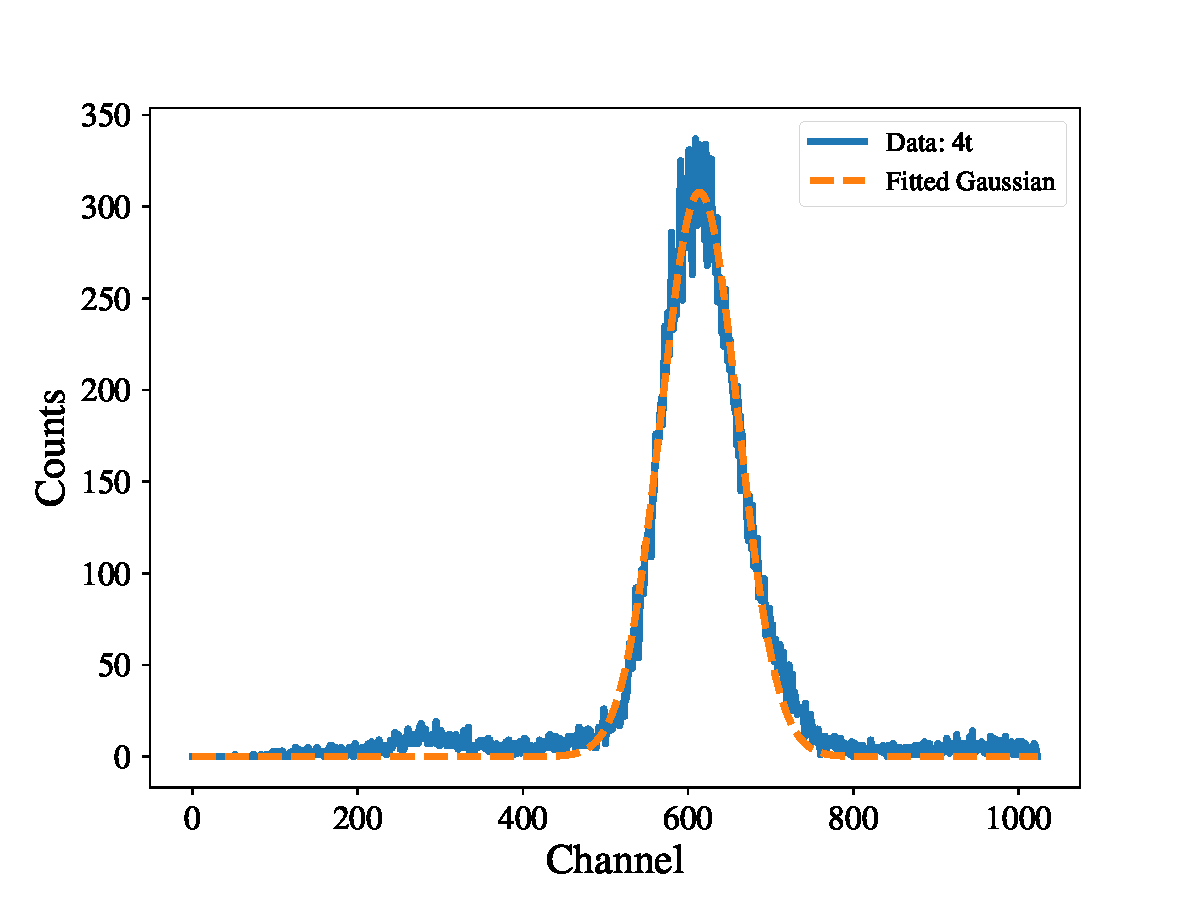
\includegraphics[width=0.7\textwidth]{../plot/Fitted_4t.pdf}
        \caption{4片铝吸收片测量结果拟合图\label{fig:Fitted_4t}}
    \end{figure}
    \begin{figure}[htbp]
        \centering
        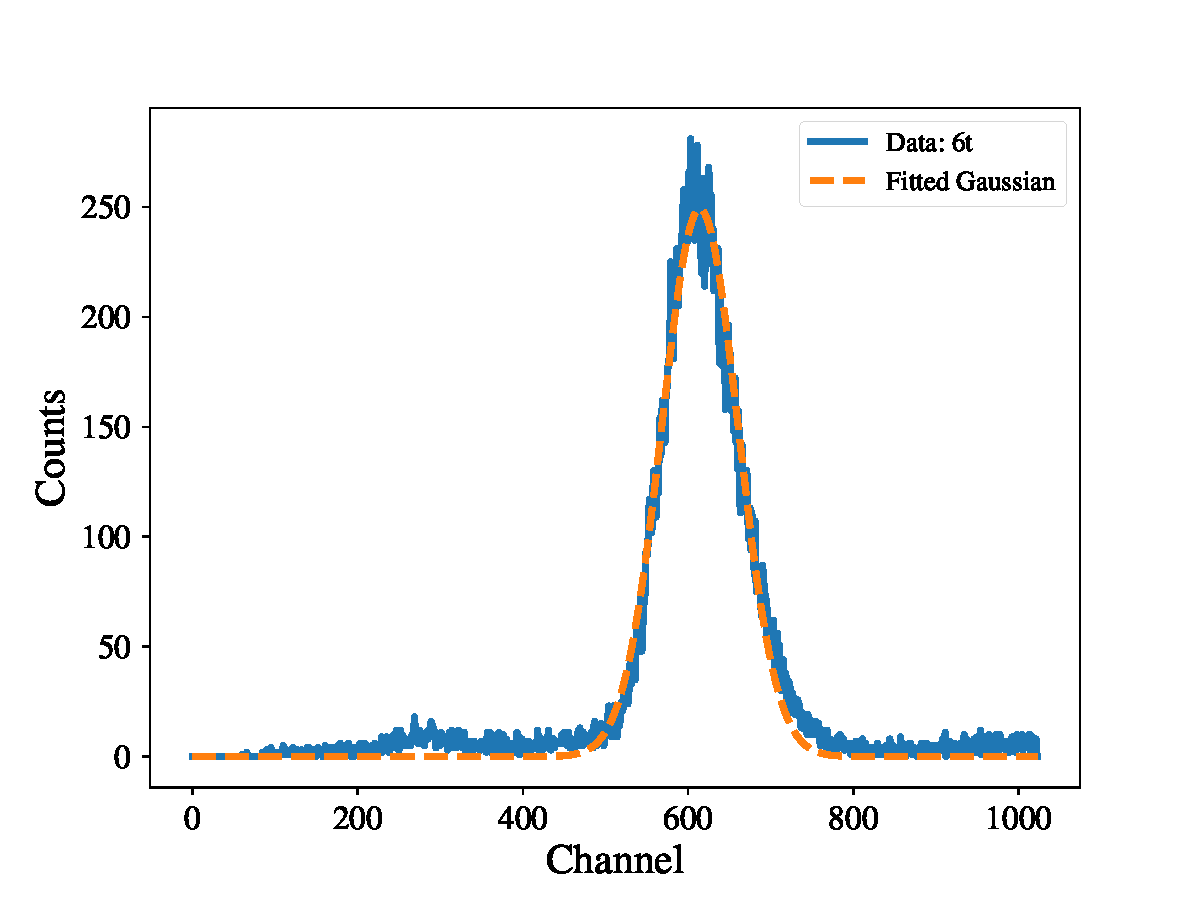
\includegraphics[width=0.7\textwidth]{../plot/Fitted_6t.pdf}
        \caption{6片铝吸收片测量结果拟合图\label{fig:Fitted_6t}}
    \end{figure}
    \begin{figure}[htbp]
        \centering
        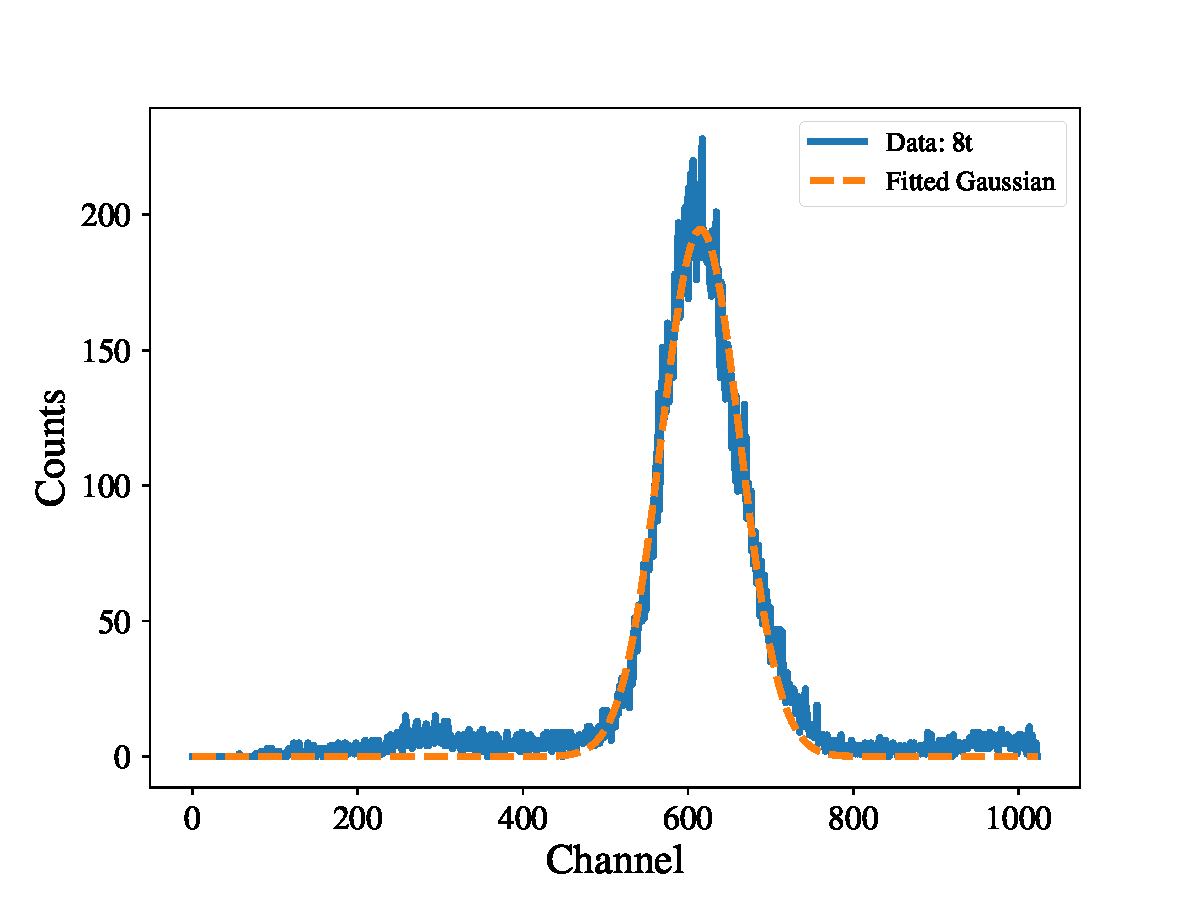
\includegraphics[width=0.7\textwidth]{../plot/Fitted_8t.pdf}
        \caption{8片铝吸收片测量结果拟合图\label{fig:Fitted_8t}}
    \end{figure}
    \begin{figure}[htbp]
        \centering
        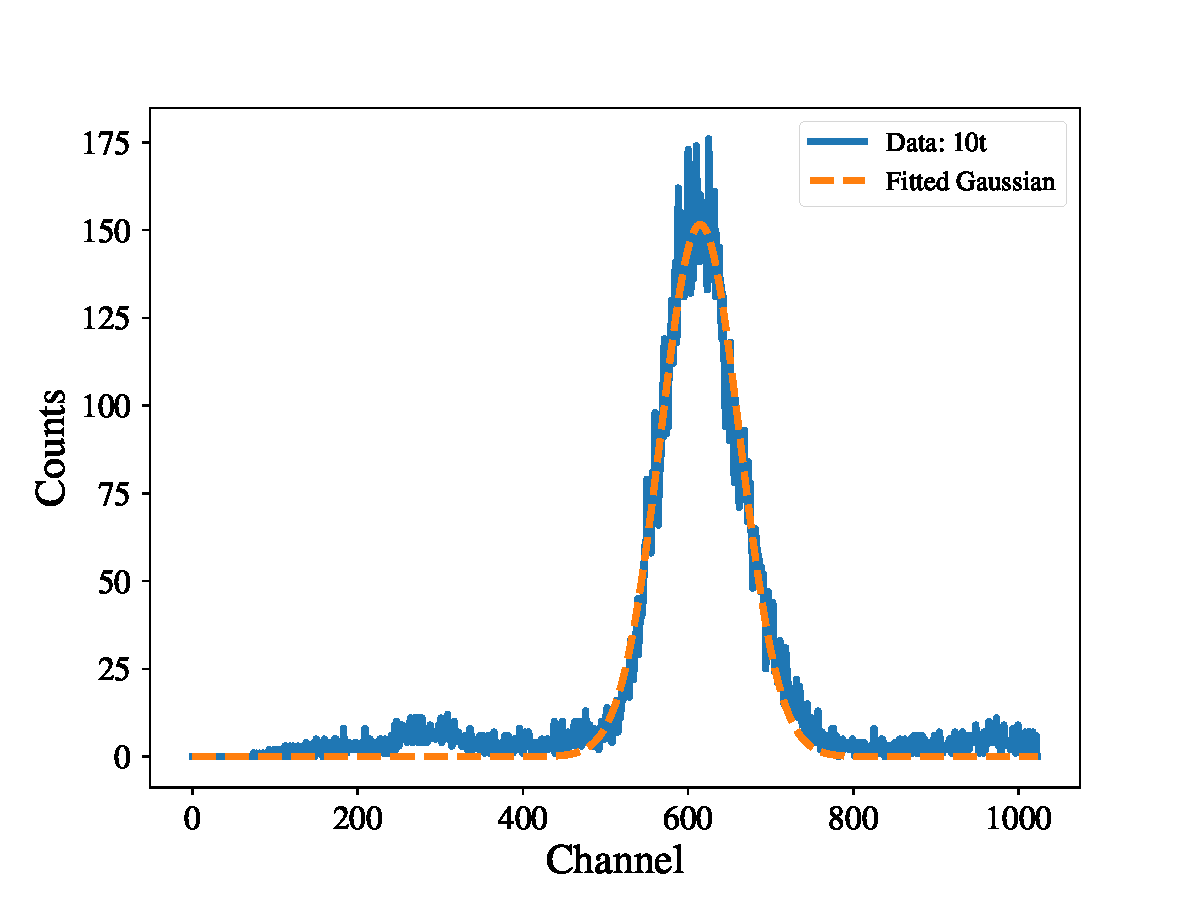
\includegraphics[width=0.7\textwidth]{../plot/Fitted_10t.pdf}
        \caption{10片铝吸收片测量结果拟合图\label{fig:Fitted_10t}}
    \end{figure}
\end{document}